\section{Sewer reservoir}\label{se:sewer_reservoir}
In this section the model for a reservior will be derived. 

In figure \ref{fig:tank_model} an illustration of a reservoir is shown.
\begin{figure}[H]
\centering
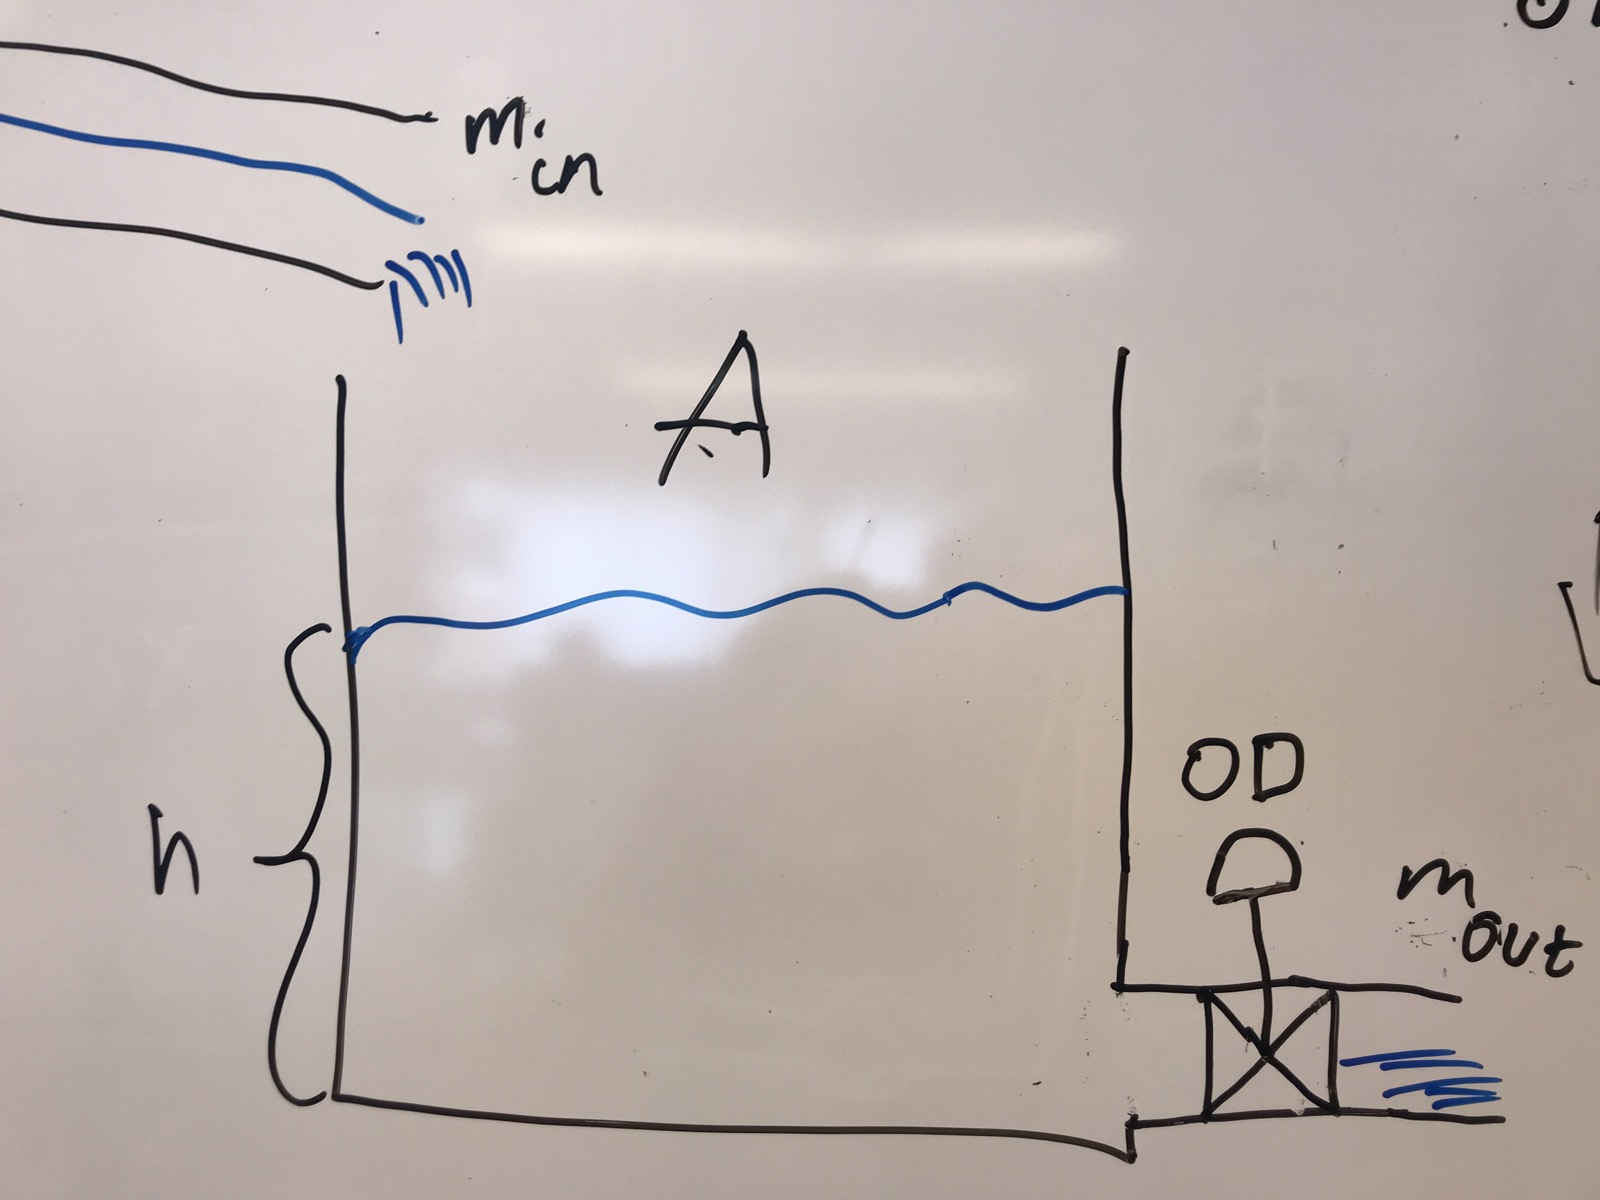
\includegraphics[width=.6\textwidth]{report/modeling/pictures/tank_model.jpg}
\caption{An illustration of a reservoir.}
\label{fig:tank_model}
\end{figure} 

This illustration will be used to derive the model for the reservior. From the left an open channel that discharges fluid into the reservoir is shown. The fluid going into the reservoir has a mass flow rate, $m_{in}$ [$\frac{kg}{sec}$]. Within the reservoir the stored fluid has a height, h [$m$], and the reservoir has a surface area, A. To the bottom right the fluid is discharged, $m_{out}$. The output mass flow is depended on the openings degree (OD) of the valve. The mass balance equation is derived in \cite{model_tank} and is given as:

%Assumption: incompressible flow

\begin{equation}
	 	\frac{dM_{cv}(t)}{dt}=\dot{m}_{in}(t)-\dot{m}_{out}(t)
\label{eq:tank_mass_balance}
\end{equation} 

Where $M_{cv}$ is the total mass within the control volume [$kg$], and $m_{in}$ and $m_{out}$ is the mass in and outflow rate of the tank $\left[\frac{kg}{s}\right]$. The mass balance can be written as $M_{cv} = \rho Ah$ where $\rho$ is the densisty $\left[\frac{kg}{m^3}\right]$, A is the area $\left[m^2\right]$ and h is the height [m]. The mass flow rate can be written as $m = \rho Q$, where Q is the flow $\left[\frac{m^3}{s}\right]$. Inserting this into equation \ref{eq:tank_mass_balance} the following is obtained:

\begin{equation}
		\frac{d(\rho Ah(t))}{dt}=\rho Q_{in}(t)-\rho Q_{out}(t)
\end{equation}

By assuming incompressible fluid such that density is constant then:

\begin{equation}\label{eq:balance_reservior}
	\rho A\frac{dh(t)}{dt}=\rho \left(Q_{in}(t)-Q_{out}(t)\right)
\end{equation}
Simplifying equation \ref{eq:balance_reservior} by dividing with $\rho A$:

\begin{equation}\label{eq:balance_reserviorv2}
	\frac{dh(t)}{dt}=\frac{1}{A} \left(Q_{in}(t)-Q_{out}(t)\right)
\end{equation}

Because the output flow is depending on the OD of the valve, a model is needed to described the output flow of it. The model for the valve is derived by \cite{boysen} and is given as:
\begin{equation}\label{eq:valve_model}
	Q_{out} = kv(OD) \sqrt{\Delta p}
\end{equation}
Where kv(OD) is a function that describes the flow for different ODs. $\Delta p$ is the pressure drop across the valve [Pa]. The pressure at the bottom of the tank can be found with:

\begin{equation}\label{eq:pressure_at_depth}
 	P_{bot} = P_{top} +\rho g h
 \end{equation} 
 Where $P_{top}$ is the atmospheric pressure $[Pa]$ and g is the gravitational constant $\left[\frac{m}{s^2}\right]$. The pressure on the output side of the valve is assumed to be approximately 101,375 $kPA$ as it is an open channel. Inserting equation \ref{eq:pressure_at_depth} into equation \ref{eq:valve_model} the following is obtained:    


\begin{equation}\label{eq:valve_modelv2}
	Q_{out} = kv(OD) \sqrt{(P_0 +\rho g h)- P_0} = kv(OD) \sqrt{\rho g h} 
\end{equation}

Equation \ref{eq:valve_modelv2} can be inserted into equation \ref{eq:balance_reserviorv2} and thereby the following model for the reservoir is obtained.

\begin{equation}\label{eq:balance_reserviorv3}
	\frac{dh(t)}{dt}=\frac{1}{A} \left(Q_{in}(t)-\left(kv(OD) \sqrt{\rho g h(t)}\right)\right)
\end{equation}

Equation \ref{eq:balance_reserviorv3} then gives an expresion where change in height is given as a function of inflow, pressure and opening degree of the valve. 